\subsection{Добавляем источники ресурсов}
Начнем наполнение зон в нашем шаблоне с источников ресурсов. Заранее определимся что каждая стартовая зона будет содержать 2 золотые шахты и два источника родной маны. Одна из двух золотых шахт и один источник будут под контролем игрока со старта, остальные придется разведать и захватить в процессе игры.

Поскольку игрок может выбрать любые расы для создания сценария, нам как авторам шаблона нужно учесть это и контроллировать наполнение зон, выбирая тип источников маны с учетом выбранных рас. В этом нам также поможет список рас, поданный в функцию \texttt{getContents}.

Для удобства нашей разработки шаблона и соблюдения правила с рудниками мы вынесем их описание в отдельную функцию, которую будем использовать в описании обеих зон.
Назовем функцию \texttt{getMines} для понимания ее смысла в дальнейшем.
Функция принимает расу игрока в стартовой зоне \texttt{race} и на основании нее вернет таблицу с \hyperref[crystals]{источниками ресурсов} для зоны.
Количество золотых шахт одинаково для обеих стартовых зон, поэтому мы можем сразу указать их в локальной таблице:

\begin{figure}[H]
\lstinputlisting[firstnumber=1, firstline=1, lastline=7]{docExamples/templateExample2.lua}
\caption{Функция для описания источников ресурсов}
\end{figure}

Таблица создается локально внутри функции, а затем после наполнения данными возвращается с помощью директивы \texttt{return}. Такой формат описания выбран только для наглядности. Таблицу источников можно объявить после директивы \texttt{return} и сразу наполнить содержимым, не создавая локально.

Вызываем нашу функцию при описании содержимого каждой из стартовых зон, подавая расу игрока. Таким образом правила генерации источников будут одинаковы для обеих зон даже после изменения логики функции:

\begin{figure}[H]
\lstinputlisting[firstnumber=28, firstline=28, lastline=28]{docExamples/templateExample2.lua}
\lstinputlisting[firstnumber=36, firstline=36, lastline=36]{docExamples/templateExample2.lua}
\caption{Источники ресурсов в стартовых зонах}
\end{figure}

Полный текст шаблона выглядит так:

\begin{figure}[H]
\lstinputlisting{docExamples/templateExample2.lua}
\caption{Заготовка шаблона с золотыми шахтами}
\end{figure}

Сгенерируем карту на основе этого шаблона и убедимся что каждая зона содержит две золотые шахты, расположенные случайно:

\begin{figure}[H]
\center
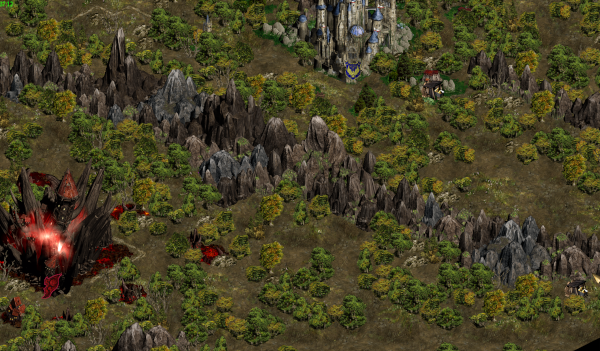
\includegraphics[width=1.0\linewidth]{docImages/scenarioWithMines.png}
\caption{Сценарий с золотыми шахтами}
\end{figure}

На миникарте видны все 4 золотые шахты, по 2 в каждой стартовой зоне:

\begin{figure}[H]
\center
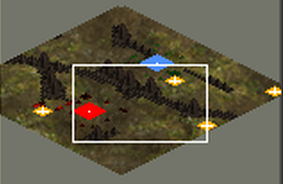
\includegraphics[width=.48\linewidth]{docImages/scenarioMinimapWithMines.png}
\caption{Миникарта с золотыми шахтами}
\end{figure}

На момент когда код функций \texttt{getContents} и \texttt{getMines} будет обработан программой генератора, список рас, присутствующих в сценарии, полностью определен, поэтому нам нужно учитывать только играбельные \hyperref[raceTypes]{расы}. Проверим каждую из 5 рас и добавим в таблицу 2 источника нужного типа:

\begin{figure}[H]
\lstinputlisting[firstnumber=1, firstline=1, lastline=19]{docExamples/templateExample3.lua}
\caption{Выбор источников ресурсов по расе игрока}
\end{figure}

Полный текст шаблона выглядит так:

\begin{figure}[H]
\lstinputlisting{docExamples/templateExample3.lua}
\caption{Шаблон с источниками ресурсов}
\end{figure}

Результаты генерации, в этот раз нам выпали Горные Кланы и Эльфы. Два источника маны рун в зоне кланов и два источника лесного эликсира у эльфов видны на миникарте:

\begin{figure}[H]
\center
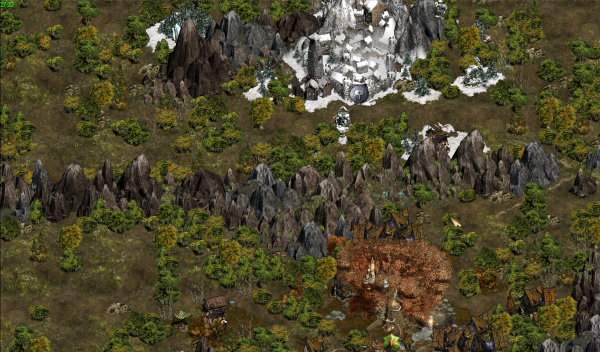
\includegraphics[width=1.0\linewidth]{docImages/scenarioWithMines2.png}
\caption{Сценарий с источниками ресурсов}
\end{figure}

\begin{figure}[H]
\center
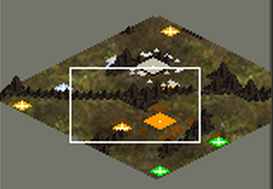
\includegraphics[width=.48\linewidth]{docImages/scenarioMinimapWithMines2.png}
\caption{Миникарта с источниками ресурсов}
\end{figure}